\paragraph{Packet Radio}

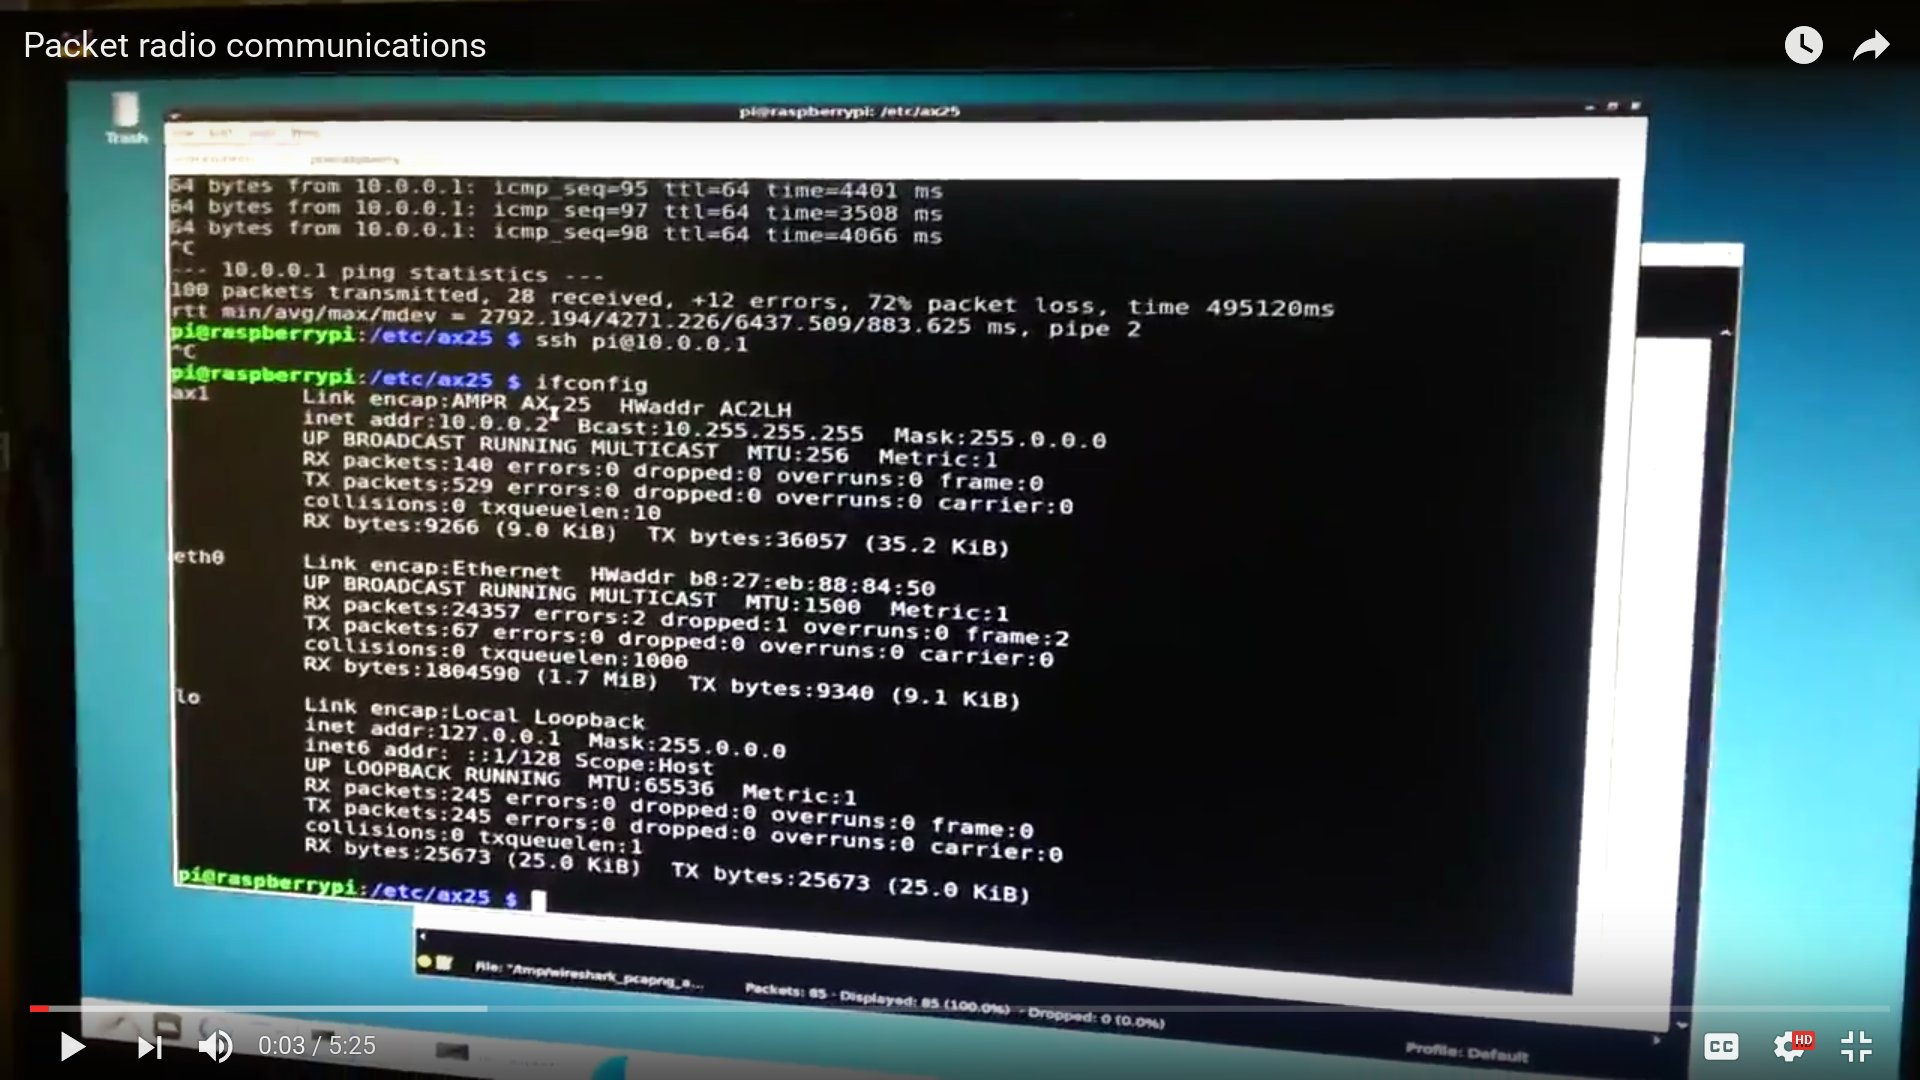
\includegraphics[width=0.7\linewidth]{files/packet_radio-01809f74970f9257a92862b82d321439.jpg}

\subparagraph{Introduction}

Packet radio is a digital mode of communication that is used by amateur radio operators. It is a form of packet switching that allows data to be sent in small packets over a radio link. Packet radio is used for a variety of purposes, including emergency communications, data transmission, and connecting to the internet.

In this section, we will show an an experiment with a simple packet radio setup using a Raspberry Pi and a Yaesu VX-8DR handheld transceiver using VHF frequencies and the AX.25 protocol.

\subparagraph{Videos}

\subparagraph{Video of Raspberry Pi Sending out Ping Packets Over Radio Using the AX25 Protocol}

\subparagraph{Video of Packet Radio using the AX25 Protocol with Raspberry Pi and Yaesu VX-8DR}

\subparagraph{Investigation Audio Drive Levels for Packet Radio}

\subparagraph{Packet Radio Websites}

This is a list of websites that provide information on packet radio and related topics:

\subparagraph{The Digital Domain of Amateur Radio - Wireless TCP/IP - Amateur Radio Digital Communications (NET-AMPRNET) AMPRNET 44.0.0.0}

\href{https://www.qsl.net/kb9mwr/wapr/tcpip/amprnet.html}{The Digital Domain of Amateur Radio - Wireless TCP/IP - Amateur Radio Digital Communications (NET-AMPRNET) AMPRNET 44.0.0.0}

\subparagraph{Using Part 15 Wireless Ethernet Devices For Amateur Radio Broadband Highspeed Amateur Multimedia Networking}

\href{https://www.qsl.net/kb9mwr/projects/wireless/plan.html}{Using Part 15 Wireless Ethernet Devices For Amateur Radio Broadband Highspeed Amateur Multimedia Networking}

\subparagraph{The WAPR TCP/IP Page}

\href{https://www.qsl.net/kb9mwr/wapr/tcpip/}{The WAPR TCP/IP Page}

\subparagraph{XASTIR - HowTo: AX.25 - Ubuntu/Debian}

\href{https://xastir.org/index.php/HowTo:AX.25\_-\_Ubuntu/Debian}{https://xastir.org/index.php/HowTo:AX.25\_-\_Ubuntu/Debian}

\subparagraph{Getting Started with Packet Radio}

\href{https://www.trinityos.com/HAM/Packet-GettingStarted/getting-started-with-packet-radio.txt}{https://www.trinityos.com/HAM/Packet-GettingStarted/getting-started-with-packet-radio.txt}

\subparagraph{Raspberry Pi \& Soundmodem -- It works!!}

\href{http://ve3bux.com/?p=825}{http://ve3bux.com/?p=825}

\subparagraph{AX.25 Soundmodem}

\href{https://www.george-smart.co.uk/wiki/AX25\_Soundmodem}{https://www.george-smart.co.uk/wiki/AX25\_Soundmodem}

\subparagraph{Digital Modes for Ham Radio}

\href{http://www.trinityos.com/HAM/CentosDigitalModes/hampacketizing-centos.html\#3a.ax25code}{http://www.trinityos.com/HAM/CentosDigitalModes/hampacketizing-centos.html\#3a.ax25code}

\subparagraph{Starting with AX.25}

\href{http://k4gbb.no-ip.org/docs/StartingAX25.html}{http://http://k4gbb.no-ip.org/docs/StartingAX25.html}

\subparagraph{Sound Card Packet Radio}

\href{http://www.qsl.net/kb9mwr/wapr/sound-card-packet.html}{http://www.qsl.net/kb9mwr/wapr/sound-card-packet.html}

\subparagraph{Direwolf User Guide}

\href{https://github.com/wb2osz/direwolf/blob/master/doc/User-Guide.pdf}{doc/User-Guide.pdf}

\subparagraph{Direwolf Configuration File Example}

\href{http://www.trinityos.com/HAM/CentosDigitalModes/etc/ax25/direwolf.conf}{http://www.trinityos.com/HAM/CentosDigitalModes/etc/ax25/direwolf.conf}

\subparagraph{More Packet Radio Links}

\href{https://andrewmemory.wordpress.com/category/packet/}{https://andrewmemory.wordpress.com/category/packet/}

\subparagraph{Fedora Amateur Radio Guide}

\href{https://jfearn.fedorapeople.org/fdocs/en-US/Fedora/19/html-single/Amateur\_Radio\_Guide/index.html}{https://jfearn.fedorapeople.org/fdocs/en-US/Fedora/19/html-single/Amateur\_Radio\_Guide/index.html}

\subparagraph{Tigertronics}

\href{http://www.tigertronics.com}{http://www.tigertronics.com/}

\subparagraph{VNC Server at Startup on Raspberry Pi}

\href{https://learn.adafruit.com/adafruit-raspberry-pi-lesson-7-remote-control-with-vnc/running-vncserver-at-startup}{https://learn.adafruit.com/adafruit-raspberry-pi-lesson-7-remote-control-with-vnc/running-vncserver-at-startup}

\subparagraph{Ham Radio Band Plan}

\href{http://www.hamuniverse.com/hfbandplan.html}{http://www.hamuniverse.com/hfbandplan.html}

\subparagraph{Linux Amateur Radio AX.25 HOWTO}

\href{http://www.tldp.org/HOWTO/AX25-HOWTO/index.html}{http://www.tldp.org/HOWTO/AX25-HOWTO/index.html}

\subparagraph{AX.25 Libraries, Utilities \& Applications}

\href{http://f6bvp.org/ax25-libraries-utilities-applications/}{http://f6bvp.org/ax25-libraries-utilities-applications/}

\subparagraph{F6CTE's AX.25 Resources}

\href{http://f6cte.free.fr/index\_anglais.htm}{http://f6cte.free.fr/index\_anglais.htm}

\subparagraph{Soundmodem AX.25 Packet Modem}

\href{http://www.qbjnet.com/packet.html\#soundmodem}{http://www.qbjnet.com/packet.html\#soundmodem}

\subparagraph{Netcat Cheat Sheet}

\href{https://www.sans.org/security-resources/sec560/netcat\_cheat\_sheet\_v1.pdf}{https://www.sans.org/security-resources/sec560/netcat\_cheat\_sheet\_v1.pdf}

\subparagraph{RMS Express Installation on Linux}

\href{https://dcj21net.wordpress.com/2016/06/17/install-rms-express-linux/}{https://dcj21net.wordpress.com/2016/06/17/install-rms-express-linux/}

\subparagraph{AX.25 HOWTO - Table of Contents}

\href{http://www.tldp.org/HOWTO/AX25-HOWTO/x1449.html}{http://www.tldp.org/HOWTO/AX25-HOWTO/x1449.html}

\subparagraph{FPAC USER Manual}

\href{http://www.n4zkf.com/files/fadca/FPACUSER-Manual.html}{http://www.n4zkf.com/files/fadca/FPACUSER-Manual.html}

\subparagraph{AXCALL User Manual}

\href{http://manpages.ubuntu.com/manpages/trusty/man1/axcall.1.html}{http://manpages.ubuntu.com/manpages/trusty/man1/axcall.1.html}

\subparagraph{Xastir - An Amateur Packet Radio Terminal Node Controller and APRS Client}

\href{https://github.com/Xastir/Xastir}{https://github.com/Xastir/Xastir}

\subparagraph{slsnif}

\href{https://linux.die.net/man/1/slsnif}{https://linux.die.net/man/1/slsnif}

\subparagraph{Virtual Serial Port for Linux}

\href{https://stackoverflow.com/questions/52187/virtual-serial-port-for-linux}{https://stackoverflow.com/questions/52187/virtual-serial-port-for-linux}